\documentclass[table]{beamer}
%\useoutertheme{infolines}
\usepackage{multirow}
\usepackage{textpos}
\usepackage{graphicx}
\usepackage{lipsum}
%\graphicspath{{images/}}
\usepackage{verbatim} % For using /begin{comment}; /end{comment}

% Font
%\setbeamerfont{frametitle}{series=\bfseries} % Frame titles should be bold
\usepackage{lmodern}

\setbeamertemplate{itemize items}[circle]
\setbeamertemplate{itemize subitems}[circle]

% Colors
\definecolor{oj}{rgb}{1.0,0.65,0.0}
\definecolor{cblue}{rgb}{0.39,0.58,0.93}
\definecolor{amethyst}{rgb}{0.6, 0.4, 0.8}

\definecolor{lightgrey}{rgb}{0.75, 0.75, 0.80}
\definecolor{tangerine}{rgb}{1.0, 0.6, 0.4}
\definecolor{arylyellow}{rgb}{0.91, 0.84, 0.42}
\definecolor{gsa}{rgb}{0.66, 0.89, 0.63}
\definecolor{aqua}{rgb}{0.5, 1.0, 0.83}
\definecolor{bblue}{rgb}{0.67, 0.9, 0.93}


%\usepackage{tikz}
%\usebackgroundtemplate{%
%\tikz\node[opacity=0.3]{%
%\setbeamercolor{background canvas}{bg=black}
%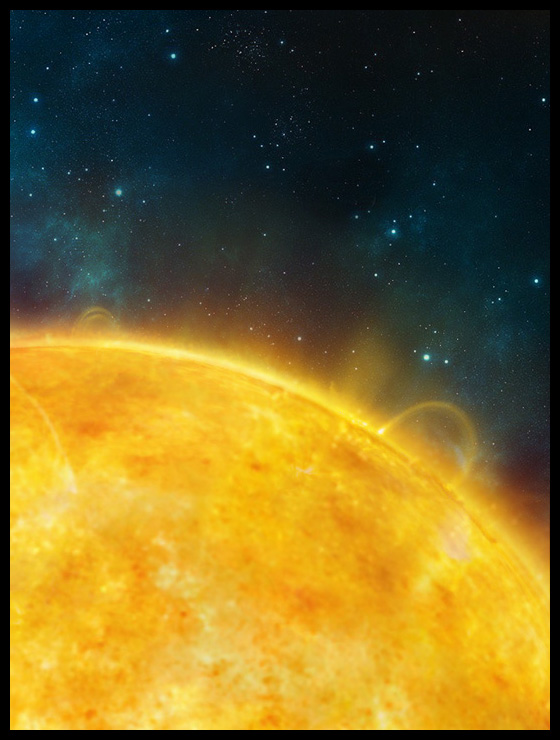
\includegraphics[height=\paperheight,width=\paperwidth]{awesome.jpg}};}

%\setbeamertemplate{background}{%

%\setbeamercolor{normal text}{bg=black, fg=white}

%\setbeamercolor{bgcolor}{fg=black,bg=red!20}
%\setbeamercolor{bgcolor}{bg=black}
%\setbeamercolor{bgcolor}{bg=red!20}

\setbeamercolor{background canvas}{bg=black}
\setbeamercolor{normal text}{fg=white}
\setbeamercolor{title}{fg=arylyellow}
\setbeamercolor{frametitle}{fg=tangerine}
\setbeamercolor{framesubtitle}{fg=gsa}
\setbeamercolor{block title}{fg=aqua}
\setbeamercolor{description item}{fg=amethyst}
\setbeamercolor{itemize item}{fg=amethyst} % all frames will have red bullets
\setbeamercolor{itemize subitem}{fg=amethyst} % all frames will have red bullets
\setbeamercolor{enumerate item}{fg=amethyst} % all frames will have red bullets
%\setbeamercolor{block title}{fg=green}

\newcommand\Wider[2][3em]{%
    \makebox[\linewidth][c]{%
       \begin{minipage}{\dimexpr\textwidth+#1\relax}
           \raggedright#2
       \end{minipage}%
    }%
}

\title{\textbf{Coronal Seismology}}
\subtitle{\textbf{ASTR 598}}
\date{\textbf{Spring 2016}}
\author{\textbf{Laurel Farris}}

\begin{document}

{\usebackgroundtemplate{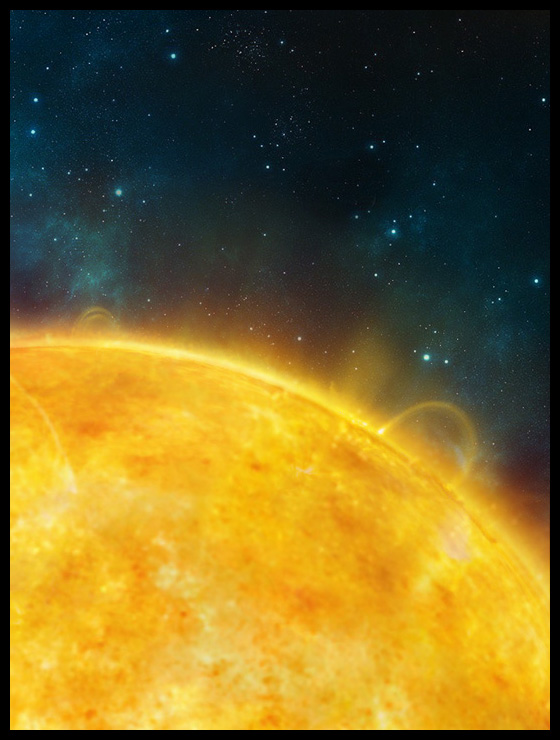
\includegraphics[width=\paperwidth]
    {awesome.jpg}}
\begin{frame}
    \titlepage{}
\end{frame}}%-------------------------------------------------------------%
\begin{comment}
\begin{frame}{template}
    \begin{columns}
        \column{0.5\textwidth}
        % ...
        \column{0.5\textwidth}
        % ...
    \end{columns}
\end{frame}%-------------------------------------------------------------%
\end{comment}
\begin{frame}{Coronal seismology}{Technique and motivation}
    Motivation:
    \begin{itemize}
        \item Mystery of coronal heating
        \item Space weather prediction
    \end{itemize}
    Properties of the solar corona that are difficult to measure:
    \begin{itemize}
        \item magnetic field strength, $\vec{B}$
        \item density
        \item Alfv\'en velocity
    \end{itemize}
    Solution: coronal seismology
    \begin{enumerate}
        \item Observe disturbances (triggered by flares, footpoint motions)
        \item Measure, e.g.\ period, velocities, timescales
        \item Identify the type of wave or mode (MHD theory; stay tuned)
        \item Extract coronal parameters from equations
    \end{enumerate}
    Other questions:
    \begin{itemize}
        \item How are these disturbances initiated?
        \item How are they damped, and what determines the timescales?
    \end{itemize}
\end{frame}%-------------------------------------------------------------%
\begin{frame}{Magnetohydrodynamics (MHD)}{Theory}
    %[Relationship between size and decay time].
    %[Something about Asc, TRACE, etc.]
    \begin{columns}
        \column{0.45\textwidth}
        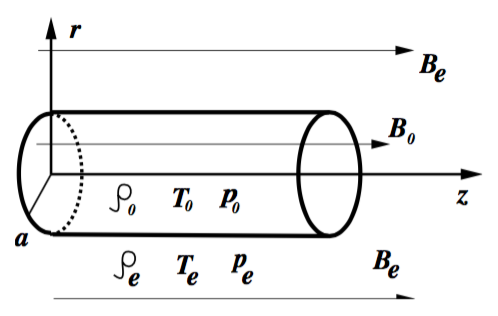
\includegraphics[width=\textwidth]{cylinder.png}\\
        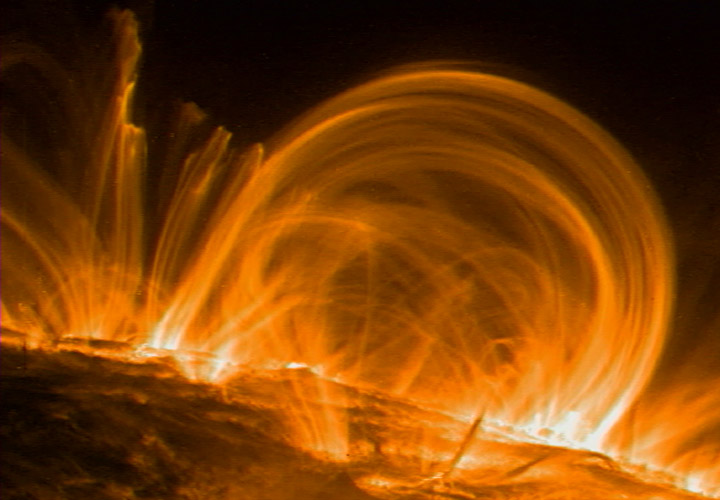
\includegraphics[width=\textwidth]{loop.jpg}
        \column{0.55\textwidth}
        \begin{itemize}
            \item Loop modeled by straight flux tube in uniform magnetic field.
            %\item $ \xi(x) = \xi(r)e^{i(kz+m{\phi})} $
            \item Characteristic speeds are determined by the
                environment
            %\item Non-ideal effects: gravitational stratification,
            %    thermal conduction, radiative cooling,
            %    loop curvature, inhomogeneity in magnetic field strength
            %    (considered negligible).
        \end{itemize}
    \end{columns}
\end{frame}%-------------------------------------------------------------%
\begin{frame}{Dispersion diagram}{Solutions to dispersion relation}
    \begin{figure}
        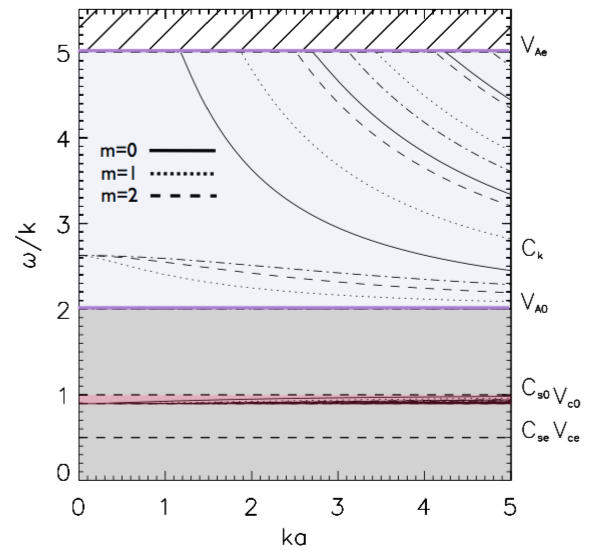
\includegraphics[width=0.65\paperwidth]{disp_diagram.png}
    \end{figure}
\end{frame}%-------------------------------------------------------------%
\begin{frame}{Magnetohydrodynamics (MHD)}{Two mode categories}
        \begin{enumerate}
            \item \textcolor{bblue}{Magnetoacoustic}
                $C_s = \sqrt{\frac{\gamma P}{\rho}}$
                \begin{itemize}
                    \item Fast $k_{A_0} < C_{fast} < C_{A_e} $
                    \item Slow $C_{T_0} < C_{slow} < C_{s_0} $
                \end{itemize}
            \item \textcolor{bblue}{Alfv\'en}
                $V_A = \frac{B}{\sqrt{\mu_0\rho}}$
        \end{enumerate}
\end{frame}%-------------------------------------------------------------%
\begin{frame}{Fast standing oscillations}{Kinks vs.\ Sausages}
    \begin{columns}
        \column{0.4\textwidth}
        \framebox{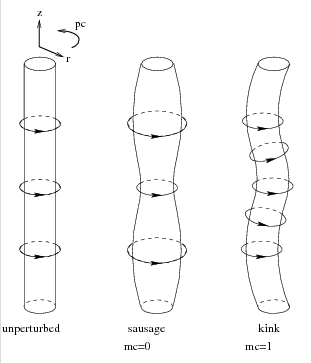
\includegraphics[width=\textwidth]{kink_saus.png}}
        \column{0.5\textwidth}
    \begin{block}{Kink}
        \begin{itemize}
            \item loop spatial displacement
            \item Asymmetric
            \item No intensity change
            \item $k\sigma \ll 1$, or $\sigma\ll\lambda$
            \item \textcolor{arylyellow}{Derive magnetic field!}
        \end{itemize}
    \end{block}
    \begin{block}{Sausage}
        \begin{itemize}
            \item No loop spatial displacement
            \item Symmetric
            \item Intensity change\\ $\rightarrow$ density change
            \item $\lambda\sim\sigma$
            \item long-wavelength limit
        \end{itemize}
    \end{block}
\end{columns}
\end{frame}%-------------------------------------------------------------%


\begin{comment}
\begin{frame}{Kink modes}{general characteristics}
    \begin{itemize}
        \item $c_k=\sqrt{\frac{\rho_oV_{Ao}^2 + \rho_cV_{Ac}^2}
            {\rho_o + \rho_c}}
            \approx V_A\sqrt{\frac{2}{1+\frac{\rho_e}{\rho_o}}} $
            in the low-$\beta$ plasma.
        \item $v_{ph} = \frac{\omega}{k} \approx C_k \gtrsim V_A $
        \item Period $P=\frac{2L}{V_A}\sqrt{\frac{1+\rho_e/\rho_o}{2}}$
            where $\lambda=2L$ ($L$ is the loop length).
            Typically, $L \approx 60-600$ Mm in the corona.
        \item Not just a single, global mode.
        \item Plasma motions around footpoints of coronal loops
        \item Rapidly damped
    \end{itemize}
\end{frame}%-------------------------------------------------------------%
\begin{frame}{Sausage modes}{The basics}
    Trapped fast modes supported by thick, dense loops because of the
    cutoff wavenumber (pfw\_2). Observe spatially resolved radio
    (see sources in pfw\_2).
\end{frame}%-------------------------------------------------------------%
\begin{frame}{Standing acoustic oscillations}
    [Insert movie here?]
    Characteristics:
    \begin{itemize}
        \item Pressure forces in opposition
        \item Period = 7--31 minutes (20 minutes from another source)
        \item Decay times = 5.7--36.8 minutes
        \item Peak velocity = 200 km/sec
    \end{itemize}
\end{frame}%-------------------------------------------------------------%
\end{comment}


\begin{frame}{Standing oscillations vs.\ propagating waves}
    \begin{itemize}
        \item In loops, propagating waves damp before
            reaching opposite footpoint.
        \item Velocity and intensity are 90$^{\circ}$ out of phase
            for standing oscillations, and are in phase for propagating
            acoustic waves.
        \item Frequencies less than the cutoff are standing oscillations,
            waves with frequency greater than the cutoff propagate into
            the chromosphere.
        \item no loop shape change or displacement
        \item near footpoints.
    \end{itemize}
\end{frame}%-------------------------------------------------------------%


\begin{comment}
\begin{frame}{Propagating acoustic waves}{Slow}
    \begin{itemize}
        \item $v_{ph}<150$ km s$^{-1}$ $\rightarrow$ slow
        \item longitudinal, compressive, anisotropic
        \item Parallel to $\vec{B}$, perturbation of $\vec{B}$ is negligible.
        \item Generated impulsively at one end of a footpoint.
        \item Only penetrate $\sim$ 10\% into loop before
            damped by thermal conduction
        \item weak dispersion in coronal conditions ($V_{A} \gg c_{s}$)
        \item 3 phases: periodic, QP, decay
        \item period = 3, 5, 10 minutes? Or 2--22 seconds? (see kink\_1),
        \item velocity: 50--200 km s$^{-1}$
        \item $c_{T} = \sqrt{\frac{c_{s}^2v_{A}^2}{c_{s}^2 + v_{A}^2}} $
            propagate sub-sonically at $c_{T}$, which is less than $c_{s}$
        \item ``large'' amplitude, max in top of chromosphere
        \item Observed using spectroscopy (intensity variations in
            EUV emission  and Doppler shifts)
    \end{itemize}
\end{frame}%-------------------------------------------------------------%
\begin{frame}{Propagating acoustic waves}{Fast}
    \begin{itemize}
        \item $v_{ph}>150$ km s$^{-1}$ $\rightarrow$ fast
            (\emph{or} transverse standing waves).
        \item Quasi-isotropic
        \item Driven by magnetic forces + plasma pressure forces
        \item Compressive (magnetic sound wave)
        \item Speed: $c_{F} = \sqrt{c_{s}^2 + v_{A}^2} $
        \item Moreton waves in the chromosphere
        \item Fast EUV waves in the corona
    \end{itemize}
\end{frame}%-------------------------------------------------------------%
\end{comment}
\begin{frame}{Torsional modes}{aka.\ Alfv\'en wave}
    Properties:
    \begin{itemize}
        \item m$=$0 (Axisymmetric, or azimuthally symmetric)
        \item transverse (shear) perturbations
        \item Parallel to $\vec{B}$
        \item Driving force: magnetic tensioin
        \item incompressible
        \item velocity: $v_{A} = \frac{B}{\mu_{o}\rho}$;
            $\sim$ 1000 km s$^{-1}$ in the corona
    \end{itemize}
    How to observe:
    \begin{itemize}
        \item Only get Doppler shifts from \emph{long}-period waves
            ($>$ a few minutes).
        \item Measure additional (i.e.\ non-thermal) broadening
            of coronal emission lines; indirect way to observe short-period waves.
        \item Spatial variation in Doppler shift for long periods.
            Gyrosynchrotron emission in radio regime.
    \end{itemize}
    Effects of twisting:
    \begin{itemize}
        \item Coupling of various MHD modes
    \end{itemize}
\end{frame}%-------------------------------------------------------------%
\begin{frame}{OBSERVATIONS FROM HINODE/EIS OF INTENSITY OSCILLATIONS
        ABOVE A BRIGHT POINT\@: SIGNATURE OF THE LEAKAGE OF ACOUSTIC
    OSCILLATIONS IN THE INNER CORONA}{A. K. Srivastava and B. N. Dwivedi}
    \begin{columns}
        \column{0.5\paperwidth}
        [insert plot/image here]
        \column{0.5\paperwidth}
        \begin{itemize}
            \item He{\footnotesize II} 256 \AA{} (TR and low corona)
            \item Fe{\footnotesize XV} 195 \AA{} (Upper corona)
        \end{itemize}
    \end{columns}
\end{frame}%-------------------------------------------------------------%
\begin{frame}{Another example}
    What observed and how, values measured, other parameters derived,
    mode identified, etc.
\end{frame}%-------------------------------------------------------------%
\begin{frame}{A third example}
\end{frame}%-------------------------------------------------------------%
\begin{frame}{Important Properties}
\begin{center}
    \begin{tabular}{c|c|c|c|}
    \cline{2-4} & {\textbf{period}} &
        {\textbf{decay time}} &
        {\textbf{velocity}}\\
    \hline \multicolumn{0}{|c|}{kink osc} & value & value & value\\
    \hline \multicolumn{0}{|c|}{sausage osc} & value & value & value\\
    \hline \multicolumn{0}{|c|}{acoustic osc} & 20 m & 5--30 m & 200 km s$^{-1}$\\
    \hline \multicolumn{0}{|c|}{acoustic waves} & value & value & value\\
    \hline \multicolumn{0}{|c|}{fast waves} & value & value & value\\
    \hline \multicolumn{0}{|c|}{torsional modes} & 10 m & value &
        1000 km s$^{-1}$\\
    \hline
    \end{tabular}
\end{center}
\end{frame}%-------------------------------------------------------------%
{%
\setbeamercolor{background canvas}{bg=black}
\setbeamertemplate{background}{%
\parbox[c][\paperheight][c]{\paperwidth}{%
\centering
%\hspace{3cm}
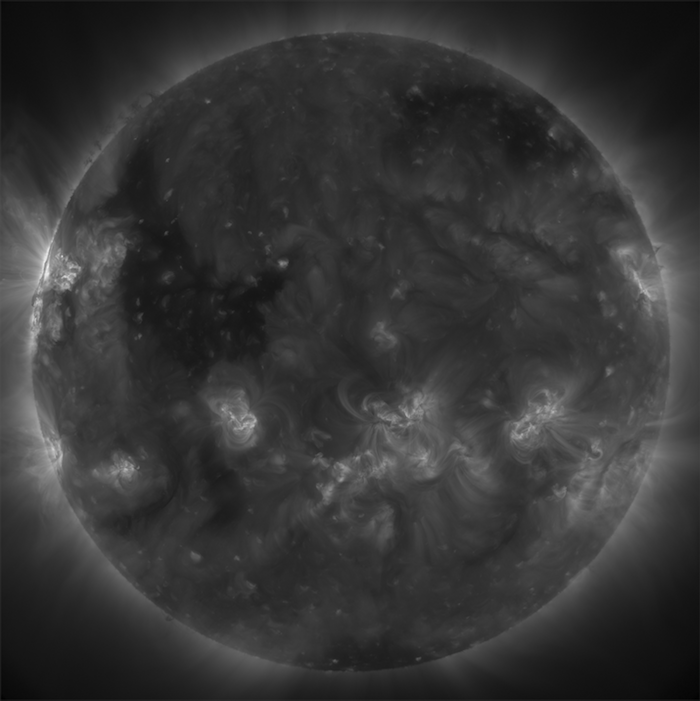
\includegraphics[height=\paperheight]{figures/full_disk.png}}}
\begin{frame}{Research}{AIA/SDO}
\end{frame}}%------------------------------------------------------------%
\begin{comment}
\begin{frame}
    Fe {\footnotesize XII, XXIV}\\
    193 \AA{}\\
    July 2012\\
    11--12 pm\\
\end{frame}
\end{comment}
\begin{frame}[c]{Research}{[Looks nicer than white background]}
    \includegraphics[width=0.7\paperwidth]{figures/bp1.png}
\end{frame}%-------------------------------------------------------------%
\begin{frame}[c]{Research}
    \includegraphics[width=0.8\paperwidth]{figures/bp1_image.png}
\end{frame}%-------------------------------------------------------------%
\begin{frame}[c]{Research}
    \framebox{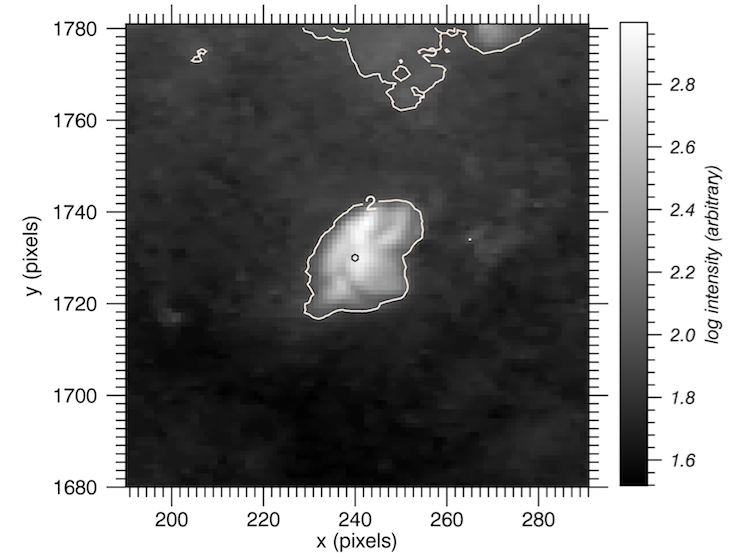
\includegraphics[width=0.8\paperwidth]{figures/bp1_contour.png}}
\end{frame}%-------------------------------------------------------------%
\begin{frame}[c]{Research}{Add BP pic in corner}
    \Wider[4em]{%
    \begin{center}
        \framebox{\includegraphics[width=0.9\paperwidth]{figures/bp1_cool2.png}}
    \end{center}}
\end{frame}%-------------------------------------------------------------%
\begin{frame}{Research}
    \begin{center}
        \includegraphics[width=0.8\paperwidth]{figures/lightcurve3.png}
    \end{center}
\end{frame}%-------------------------------------------------------------%
\begin{frame}{Acknowledgements}
\end{frame}%-------------------------------------------------------------%

\end{document}
